\chapter{Chapter Title}

\section{Text Section}

Text Text Text Text Text Text Text Text Text Text Text Text Text Text Text Text Text.


\section{Figure Section}

\begin{figure}[H]
\begin{center}
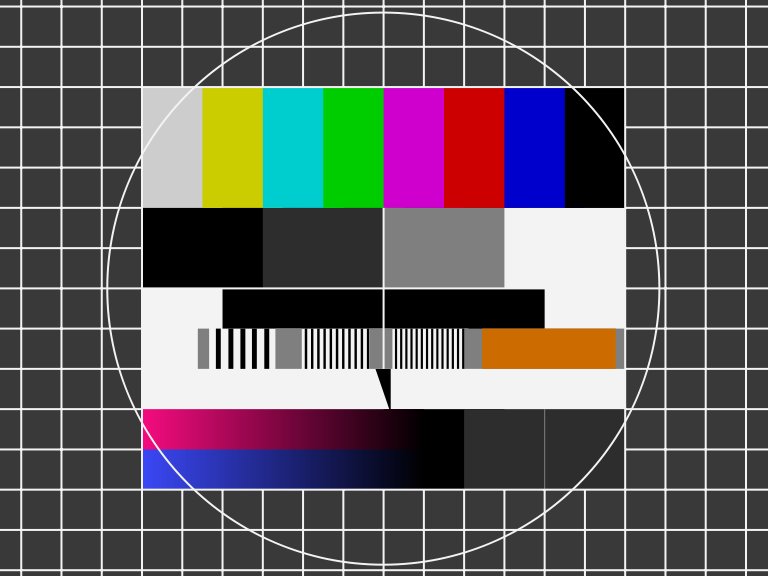
\includegraphics[width=0.8\textwidth]{./Images/test_1.png}
\end{center}
\caption{Figure description}
\end{figure}


\section{Itemize Section}

\begin{itemize}
\item text
\item text
\item text
\item text
\item text
\end{itemize}


\section{Verbatim Section}

\begin{verbatim}
text code
\end{verbatim}


\section{Lstlisting Section}

\begin{lstlisting}[language=bash, frame=single]
text code
\end{lstlisting}


\section{Cite Section}

text \cite{name1}.


\section{Two Figure Comparison Section}

\begin{figure}[H]
        \centering
        \begin{subfigure}[b]{0.5\textwidth}
                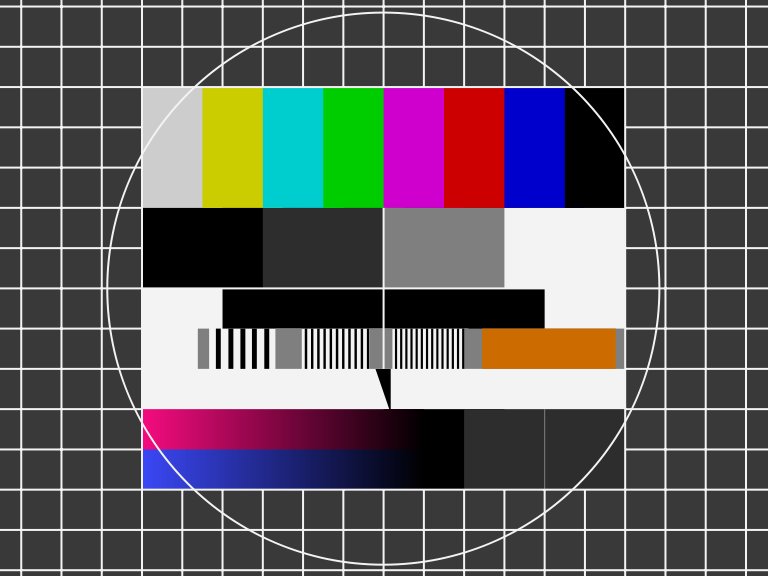
\includegraphics[width=\textwidth]{./Images/test_1.png}
                \caption{\scriptsize Comparison 1}
        \end{subfigure}%
        ~ %add desired spacing between images, e. g. ~, \quad, \qquad, \hfill etc.
          %(or a blank line to force the subfigure onto a new line)
        \begin{subfigure}[b]{0.5\textwidth}
                
\includegraphics[width=\textwidth]{./Images/test_2.png}
                \caption{\scriptsize Comparison 2}
        \end{subfigure}
\end{figure}


\section{Table Section}

\begin{table}[h]                        
\begin{center}		                    % center table
\rowcolors{1}{white}{lightcyan}			% \rowcolors{<starting row>}{<odd color>}{<even color>}
\begin{tabular}[c]{|l|c|r|}             % three columns with vertical lines
										% [b]: bottom
										% [c]: center (default)
										% [t]: top
										% l: left-justified column
										% c: centered column
										% r: right-justified column
										% |: vertical line
										% ||: double vertical line
										% p{'width'}: paragraph column with text vertically aligned at the top
										% m{'width'}: paragraph column with text vertically aligned in the middle (requires array package)
										% b{'width'}: paragraph column with text vertically aligned at the bottom (requires array package)
										% \newline: start a new line within a cell (in a paragraph column)
										% \cline{i-j}: partial horizontal line beginning in column i and ending in column j

\hline                           % inserts a horizontal line
\rowcolor{lightblue}
\textbf{header1} & \multicolumn{2}{c|}{\textbf{header2}}\\ % & separating columns
\cline{2-3}
\hline \hline                           % insert two horizontal lines
text & text & text\\          			% \\ start new row
\hline                                  % insert a horizontal line
text & text & text\\          			% \\ start new row
\hline                                  % insert a horizontal line
text & text & \cellcolor{yellow} text\\
\hline \hline                           % insert two horizontal lines

\end{tabular}
\caption[Table Description]{Table Description}
\end{center}
\end{table}